\chapter{Validation}
\label{ch:validation}

\ac{SA} always returns \emph{some} design, so its results are only meaningful if every link of the
chain is checked: the simulator must be correct, the algorithm must find optima that are known, the
problem must leave something to optimise, the algorithm must beat blind sampling, its results must
agree with the literature, its choice of fleet size must be the right one, and its designs must not
be artefacts of the coarse model. Table~\ref{tab:valplan} lists the seven checks and the rest of the
chapter reports them. All numbers are produced by \texttt{experiments/validate.py}; its full log,
every run's best design and convergence curve, and the run settings are saved in
\texttt{results/validation/}. The objective uses a fixed reference fleet of ten spacecraft, so
fleets larger than ten remain penalised consistently across all cases.

\begin{table}[htbp]
\centering
\caption{Validation plan}
\label{tab:valplan}
\footnotesize
\begin{tabularx}{\textwidth}{@{}p{0.7cm}p{3.3cm}X@{}}
\toprule
& Check & Question answered \\
\midrule
V1 & physics tests & Does the simulator agree with hand calculations? \\
V2 & known optima & Does \ac{SA} find the known minimum of standard test functions? \\
V3 & saturation & Do random fleets already cover everything (nothing to optimise)? \\
V4 & \ac{SA} vs random search & Is \ac{SA} significantly better than blind sampling with the same budget? \\
V5 & literature comparison & Under the assumptions of published work, do we reach the same coverage? \\
V6 & forced fleet size & Is the number of spacecraft \ac{SA} chooses the best one? \\
V7 & finer mesh & Do the designs keep their coverage on a four times finer asteroid model? \\
\bottomrule
\end{tabularx}
\end{table}

\section{V1: the simulator obeys physics}
\label{sec:v1}
An automated test suite (90 tests, run with every change of the code) checks the simulator against
hand calculations (Table~\ref{tab:v1}) and checks the pipeline itself: decoding and encoding of
the decision vector, every constraint and the repair operator, the penalty, the fixed-$N$ mode,
the cost terms, and the bookkeeping of the algorithms.

\begin{table}[htbp]
\centering
\caption{V1: physics checks (selection)}
\label{tab:v1}
\footnotesize
\begin{tabularx}{\textwidth}{@{}Xp{4.0cm}p{2.6cm}@{}}
\toprule
Check & Expected & Simulator \\
\midrule
Kepler solver residual, $e\le0.5$ & $<10^{-10}$ & $<10^{-10}$ \\
Circular orbit radius along the orbit & constant & constant \\
Orbital period at $a=35$\,km (Eros) & $2\pi\sqrt{a^3/\mu}=17.1$\,h & 17.1\,h \\
Energy and angular momentum along an orbit & constant & constant to 0.1\,\% \\
$\Delta V$ of a $50\rightarrow30$\,km transfer & Hohmann formula & identical \\
Usable range of the $6^\circ$ camera at 3\,m/pixel & 58.6\,km & 58.6\,km \\
Facet hidden behind terrain (concave test mesh) & not visible & not visible \\
Facet behind a blocking plate, Sun behind the plate & shadowed & shadowed \\
Eclipse behind the asteroid, battery drain & hand-computed cases & identical \\
\bottomrule
\end{tabularx}
\end{table}

\section{V2: SA finds known optima}
\label{sec:v2}
Because the \ac{SA} code is generic, it can be run unchanged on standard test functions whose global
minimum is known ($f=0$ at $\mathbf{x}=\mathbf{0}$): the smooth sphere function in five dimensions,
and the highly multi-modal Rastrigin function and the Ackley function, each in two and five dimensions
(Table~\ref{tab:v2}, 10 runs of 10\,000 evaluations each, default parameters).

\begin{table}[htbp]
\centering
\caption{V2: \ac{SA} on test functions with known minimum 0 (10 runs of 10\,000 evaluations)}
\label{tab:v2}
\footnotesize
\begin{tabular}{@{}lccccc@{}}
\toprule
Function & Dim. & Best & Mean & Worst & Runs with $f<0.1$ \\
\midrule
Sphere & 5 & 1.2e-03 & 2.5e-03 & 4.0e-03 & 100\,\% \\
Rastrigin & 2 & 7.8e-05 & 2.1e-02 & 1.2e-01 & 90\,\% \\
Rastrigin & 5 & 6.8e-03 & 4.7e-01 & 2.0e+00 & 70\,\% \\
Ackley & 2 & 2.8e-03 & 1.2e-02 & 2.4e-02 & 100\,\% \\
Ackley & 5 & 9.2e-03 & 1.9e-02 & 3.5e-02 & 100\,\% \\
\bottomrule
\end{tabular}
\end{table}


\ac{SA} reaches the global minimum of the smooth functions in every run: the sphere function in five
dimensions and the Ackley function in two and five. The Rastrigin function has a regular grid of local minima around the global one: in two dimensions 9 of 10 runs reach it, in five
dimensions 7 of 10, and the other runs end in a neighbouring local minimum (mean 0.47, i.e.\ about
half a unit above the optimum). This is the expected behaviour of a single-point method with a
finite budget on a deceptive landscape, and it shows that the algorithm is implemented correctly:
it converges, it escapes local minima most of the time, and it does not stall.

\section{V3: is there anything to optimise?}
\label{sec:v3}
If random fleets already photographed almost the whole surface, any optimiser would look good. Fifty
random designs of one, three and five spacecraft were therefore flown for ten days around Eros
(Figure~\ref{fig:sat}, Table~\ref{tab:v3}).

\begin{table}[htbp]
\centering
\caption{V3: coverage of random designs flown for ten days around Eros}
\label{tab:v3}
\footnotesize
\begin{tabular}{@{}cccccc@{}}
\toprule
$N$ & Designs & Mean $C$ & Min & Max & Share with $C\ge95\,\%$ \\
\midrule
1 & 50 & 38\,\% & 0\,\% & 77\,\% & 0\,\% \\
3 & 50 & 71\,\% & 0\,\% & 96\,\% & 2\,\% \\
5 & 50 & 88\,\% & 69\,\% & 97\,\% & 14\,\% \\
\bottomrule
\end{tabular}
\end{table}


\begin{figure}[htbp]
\centering
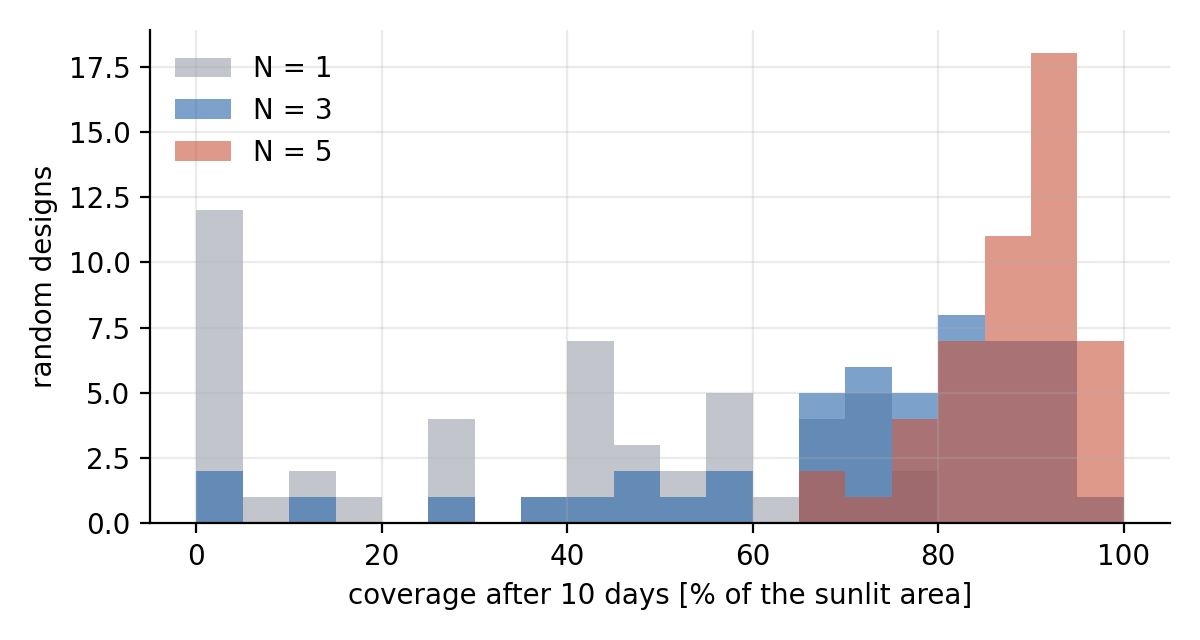
\includegraphics[width=0.7\textwidth]{Figures/fig_saturation.png}
\caption{V3: coverage reached by random designs after ten days on Eros.}
\label{fig:sat}
\end{figure}

Random fleets are far from saturating the surface. A single random spacecraft images 38\,\% of
the sunlit area on average, three image 71\,\%, and even five spacecraft flying for the full ten days
image 88\,\%. Only 2\,\% of the three-spacecraft designs and 14\,\% of the five-spacecraft designs
exceed 95\,\%, and these random designs also pay the full ten days and the cost of every spacecraft.
Good designs are therefore rare and the problem is worth optimising. The spread (from 0 to 96\,\% for
three spacecraft) also shows how strongly the orbits matter: an orbit beyond the camera range images
nothing.

\section{V4: SA against random search}
\label{sec:v4}
Random search draws designs uniformly in the same box (with the same repair) and keeps the best
feasible one; with the same number of evaluations it is the minimum any optimiser must beat. Both
methods were run five times in each of the nine settings of cases A and B. Whether \ac{SA}'s fitness
is lower is tested with the one-sided Mann--Whitney $U$ test~\cite{mann1947}, which makes no assumption about the
distribution of the results; with five runs per method the smallest possible $p$-value is
$1/\binom{10}{5}=0.004$, reached when every \ac{SA} run beats every random-search run.

\begin{table}[htbp]
\centering
\caption{V4: \ac{SA} (bold) against random search with the same budget; means over 5 runs each}
\label{tab:v4}
\scriptsize
\begin{tabular}{@{}lccccccc@{}}
\toprule
Setting & $N_{\max}$ & $J$ $\downarrow$ & $C$ [\%] $\uparrow$ & $N$ & $T$ [d] & worst SA / best RS $J$ & $p$ \\
\midrule
Eros 10 d & 5 & \textbf{0.108} / 0.167 & \textbf{95.1} / 88.8 & \textbf{2.2} / 2.8 & \textbf{2.03} / 2.95 & 0.117 / 0.159 & 0.004 \\
Eros 1 d & 5 & \textbf{0.212} / 0.309 & \textbf{88.6} / 69.7 & \textbf{3.0} / 3.0 & \textbf{0.45} / 0.47 & 0.226 / 0.285 & 0.004 \\
Eros 1 d ($N_{\max}$ 10) & 10 & \textbf{0.205} / 0.313 & \textbf{89.6} / 74.1 & \textbf{3.2} / 3.4 & \textbf{0.43} / 0.55 & 0.221 / 0.287 & 0.004 \\
Eros 12 h & 10 & \textbf{0.277} / 0.404 & \textbf{80.5} / 67.8 & \textbf{3.4} / 4.4 & \textbf{0.26} / 0.36 & 0.294 / 0.371 & 0.004 \\
Eros 6 h & 10 & \textbf{0.355} / 0.475 & \textbf{75.0} / 55.0 & \textbf{3.4} / 4.4 & \textbf{0.19} / 0.19 & 0.398 / 0.444 & 0.004 \\
Eros 2 h & 10 & \textbf{0.443} / 0.538 & \textbf{38.7} / 17.3 & \textbf{2.8} / 2.2 & \textbf{0.03} / 0.03 & 0.492 / 0.524 & 0.004 \\
Kleopatra 3 d & 5 & \textbf{0.225} / 0.310 & \textbf{74.8} / 64.3 & \textbf{2.6} / 2.8 & \textbf{0.69} / 1.10 & 0.241 / 0.300 & 0.004 \\
Kleopatra 3 d ($N_{\max}$ 10) & 10 & \textbf{0.231} / 0.316 & \textbf{76.3} / 66.2 & \textbf{2.8} / 4.4 & \textbf{0.86} / 0.89 & 0.254 / 0.303 & 0.004 \\
Kleopatra 12 h & 10 & \textbf{0.340} / 0.460 & \textbf{61.6} / 47.0 & \textbf{2.8} / 4.4 & \textbf{0.22} / 0.26 & 0.362 / 0.456 & 0.004 \\
\bottomrule
\end{tabular}
\par\smallskip
\parbox{0.95\textwidth}{\scriptsize $p$: one-sided Mann--Whitney test that \ac{SA}'s $J$ is lower. ``worst SA / best RS'': if the first number is lower, every \ac{SA} run beat every random-search run.}
\end{table}


\begin{figure}[htbp]
\centering
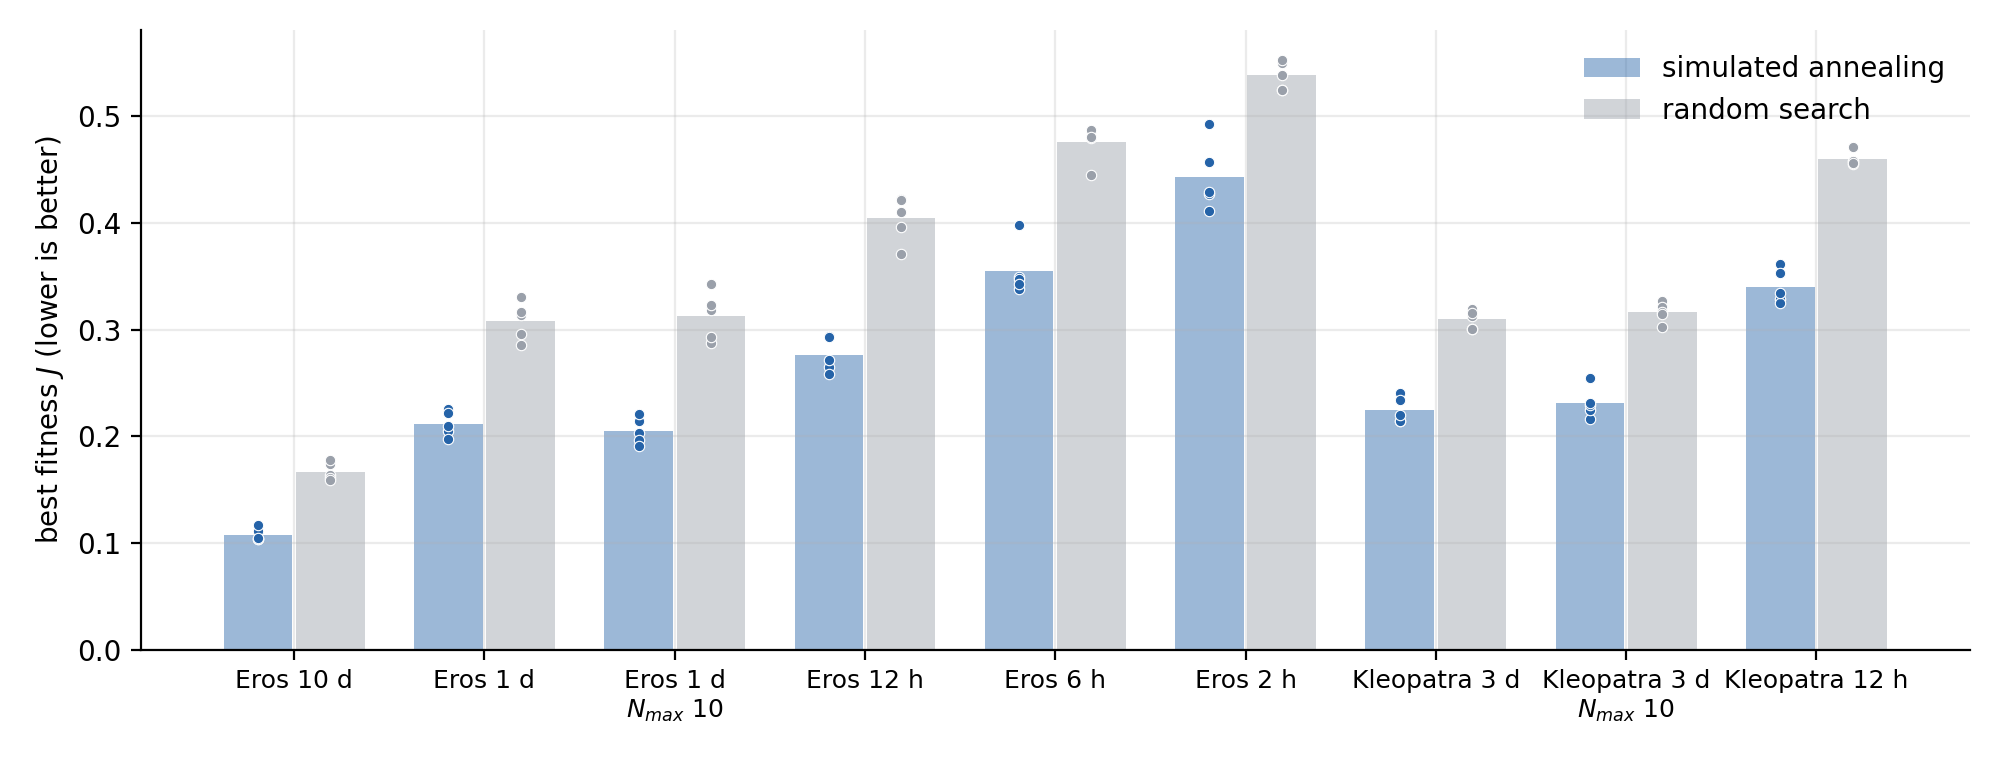
\includegraphics[width=\textwidth]{Figures/fig_sa_vs_random.png}
\caption{V4: best fitness of \ac{SA} and of random search with the same budget (bars: means, dots:
single runs; lower is better).}
\label{fig:v4}
\end{figure}

\ac{SA} wins in all nine settings and in every single run: in each setting the worst of the five
\ac{SA} runs is better than the best of the five random-search runs, so the Mann--Whitney test gives
the smallest possible $p=0.004$ nine times. The gain comes mostly from coverage, from $+6$ points in
the long ten-day Eros mission (95.1 against 88.8\,\%) to $+21$ points in the two-hour mission (38.7
against 17.3\,\%). In the short missions random search also needs more spacecraft (mean 4.4 against
3.4 at 12\,h and 6\,h on Eros) and still sees less, and in the long missions it needs longer missions
(mean 2.9 against 2.0 days for $T_{\max}=10$\,d). The advantage is smallest when the mission is long,
because the asteroid then turns many times under every orbit and almost any reasonable fleet ends
up seeing most of the surface (V3); it is largest when time is short, because \emph{where} each
spacecraft is \emph{when} decides what can be seen, and random sampling does not find such
combinations. Raising $N_{\max}$ from 5 to 10 (51 instead of 26 variables) does not hurt \ac{SA}: its
results in cases A2/A3 and B1/B2 differ by less than one standard deviation.

\section{V5: comparison with the literature}
\label{sec:v5}
The closest prior work is by Nallapu and Thangavelautham~\cite{nallapu2019}, who designed a swarm
that maps Eros during a single flyby: a genetic algorithm chose the swarm size and the positions on
a ring, and 8 spacecraft gave 100\,\% coverage at 1\,m resolution. Their model assumes the whole
surface is lit and only checks whether a facet faces the camera. In follow-up work that counts only
the sunlit side they mapped 99.1\,\% of Mars' moon Deimos~\cite{nallapu2021}. Stolfi Rosso and
Danoy~\cite{stolfi2023} tuned swarm formations around an asteroid with a genetic algorithm and found
\ac{SA} the more accurate method for on-board tuning. To compare under the same assumptions, case~D
switches the Sun and shadow tests off (every facet counts as lit) and solves the ten-day Eros mission
again.

\begin{table}[htbp]
\centering
\caption{V5: comparison with the closest prior work on Eros}
\label{tab:v5}
\scriptsize
\begin{tabular}{@{}llllll@{}}
\toprule
Work & Trajectories & Lighting & Spacecraft & Coverage (resolution) & Algorithm \\
\midrule
Nallapu \& Thangavelautham~\cite{nallapu2019} & one flyby (10 min) & ignored & 8 & 100\,\% (1\,m) & GA \\
This work, case D & orbits, $T\le10$\,d & ignored & 2, 2, 2, 2, 2 & 97.9\,\% (3\,m) & SA \\
This work, case A1 & orbits, $T\le10$\,d & Sun + shadows & 3, 2, 2, 2, 2 & 95.1\,\% (3\,m) & SA \\
\bottomrule
\end{tabular}
\end{table}


With the Sun and shadow tests switched off, \ac{SA} images 97.9--98.1\,\% of the \emph{whole} Eros
surface in every run, with two spacecraft and a mission of about 1.2 days. This is close to the
100\,\% of Nallapu and Thangavelautham, so under the same assumptions our model and optimiser give
the same answer. The remaining two percent are deep concavities that the steep 65$^\circ$ emission
limit and the occlusion test, which the reference does not apply, make invisible from any orbit.
The difference in fleet size (2 against 8) is the expected trade-off between a fast flyby, which has
to surround the body at once, and orbiting for a day, which lets the spin of Eros bring the surface to
the cameras. With realistic lighting (case A1) coverage drops to 95.1\,\% of the sunlit area, so the
lower coverage of our main results comes from the stricter lighting model, not from the optimiser.

\section{V6: is the chosen fleet size the best?}
\label{sec:v6}
In cases C1--C3 the fleet size is forced to $N=1,2,3,\dots$ and only the orbits and the duration are
optimised. If \ac{SA}'s own choice in the free problem is right, the best forced $N$ should coincide
with it (Figure~\ref{fig:v6}, Table~\ref{tab:v6}).

\begin{figure}[htbp]
\centering
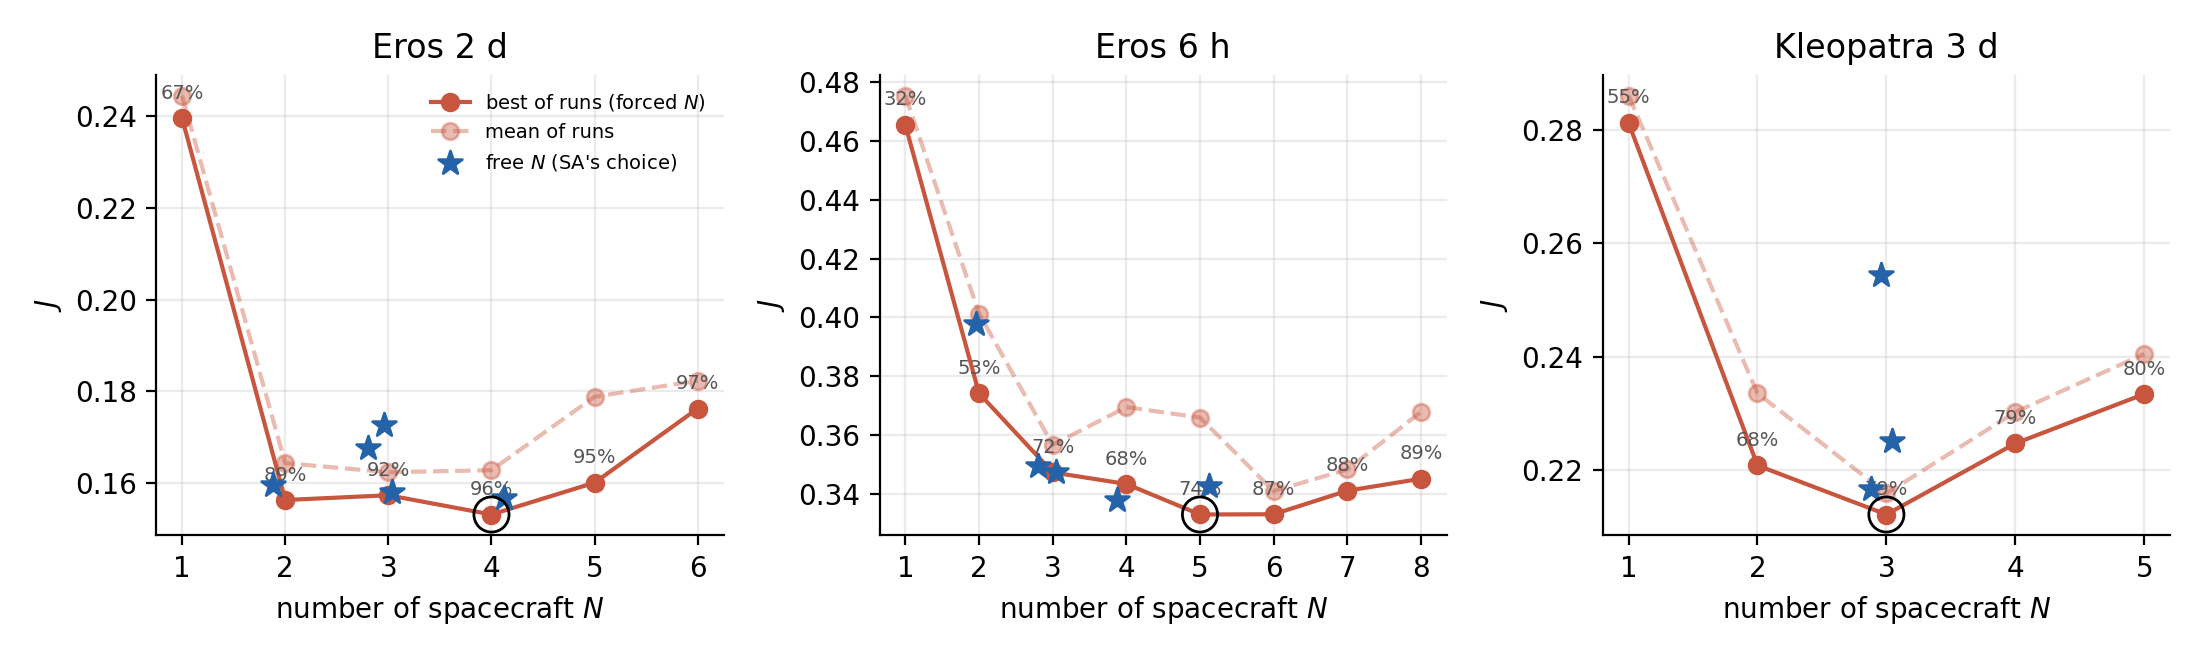
\includegraphics[width=\textwidth]{Figures/fig_fixed_n.png}
\caption{V6: best fitness when the fleet size is forced to $N$ (line) and the free-$N$ \ac{SA} runs
(stars, at the $N$ they chose).}
\label{fig:v6}
\end{figure}

\begin{table}[htbp]
\centering
\caption{V6: forced fleet size against the fleet size \ac{SA} chooses itself}
\label{tab:v6}
\scriptsize
\begin{tabular}{@{}llcccccl@{}}
\toprule
Mission & $N$ & Runs & Best $J$ & Mean $J$ & Mean $C$ & Mean $T$ & $N$ chosen \\
\midrule
Eros 2 d & 1 & 5 & 0.2395 & 0.2444 & 67.4\,\% & 14.3 h &  \\
Eros 2 d & 2 & 5 & 0.1564 & 0.1644 & 89.5\,\% & 17.0 h &  \\
Eros 2 d & 3 & 5 & 0.1574 & 0.1624 & 92.5\,\% & 15.3 h &  \\
Eros 2 d & 4 & 5 & 0.1532 & 0.1629 & 95.9\,\% & 15.6 h &  \\
Eros 2 d & 5 & 5 & 0.1601 & 0.1788 & 94.7\,\% & 12.3 h &  \\
Eros 2 d & 6 & 5 & 0.1763 & 0.1823 & 96.9\,\% & 12.6 h &  \\
Eros 2 d & free ($N_{\max}$ 10) & 5 & 0.1567 & 0.1630 & 92.4\,\% & 15.4 h & 3, 2, 3, 3, 4 \\
Eros 6 h & 1 & 5 & 0.4653 & 0.4753 & 31.6\,\% & 3.3 h &  \\
Eros 6 h & 2 & 5 & 0.3742 & 0.4013 & 53.1\,\% & 3.6 h &  \\
Eros 6 h & 3 & 5 & 0.3474 & 0.3568 & 71.6\,\% & 4.4 h &  \\
Eros 6 h & 4 & 5 & 0.3435 & 0.3696 & 68.3\,\% & 3.8 h &  \\
Eros 6 h & 5 & 5 & 0.3331 & 0.3660 & 73.5\,\% & 3.7 h &  \\
Eros 6 h & 6 & 5 & 0.3332 & 0.3411 & 86.6\,\% & 4.1 h &  \\
Eros 6 h & 7 & 5 & 0.3412 & 0.3484 & 87.9\,\% & 4.0 h &  \\
Eros 6 h & 8 & 5 & 0.3453 & 0.3679 & 88.5\,\% & 4.0 h &  \\
Eros 6 h & free ($N_{\max}$ 10) & 5 & 0.3382 & 0.3552 & 75.0\,\% & 4.5 h & 3, 4, 2, 3, 5 \\
Kleopatra 3 d & 1 & 3 & 0.2813 & 0.2861 & 54.8\,\% & 14.3 h &  \\
Kleopatra 3 d & 2 & 3 & 0.2208 & 0.2335 & 68.2\,\% & 13.7 h &  \\
Kleopatra 3 d & 3 & 3 & 0.2121 & 0.2158 & 78.6\,\% & 17.6 h &  \\
Kleopatra 3 d & 4 & 3 & 0.2247 & 0.2302 & 79.1\,\% & 15.8 h &  \\
Kleopatra 3 d & 5 & 3 & 0.2334 & 0.2405 & 79.6\,\% & 14.8 h &  \\
Kleopatra 3 d & free ($N_{\max}$ 10) & 3 & 0.2167 & 0.2321 & 77.2\,\% & 21.0 h & 3, 3, 3 \\
\bottomrule
\end{tabular}
\end{table}


Forcing the fleet size shows a clear picture: one spacecraft is always far worse, the fitness is
lowest for a moderate fleet, and large fleets become worse again because their cost outweighs the
few extra points of coverage. Near the optimum, however, the fitness is very \emph{flat}: for the
two-day Eros mission $N=2,3,4$ lie within 0.005 of each other, and for the six-hour mission $N=5$ and
$N=6$ are equal and $N=3$--$8$ lie within 0.015. Inside this flat region the choice of $N$ is
almost a tie, and the free-$N$ \ac{SA} runs land in it: for Kleopatra every run chose $N=3$, exactly
the best forced size; for the two-day Eros mission the runs chose 2--4 spacecraft and the best of
them ($J=0.1567$) is within 0.004 of the best forced design; for the six-hour mission they chose 2--5
spacecraft (best $J=0.3382$, within 0.006 of the best forced $N=5$). The free runs tend to choose
one or two spacecraft fewer than the forced optimum. Adding a spacecraft is a single move whose immediate
effect is often negative (its orbit is still untuned, but it already costs $\Delta Z=0.1$), so near
the end of the run, when the temperature is low, such moves are rarely accepted. The forced runs do
not have to take this step. This is a known weakness of a single-point method on a variable-size
problem; a population-based method that keeps several fleet sizes alive may handle it better
(the \ac{GA} of Chapter~\ref{ch:ga} starts from a population stratified over the fleet size).

\section{V7: finer asteroid model}
\label{sec:v7}
The search uses a 1\,499-facet copy of the Eros model for speed. Every best Eros design of cases A,
C, D and E, and of the random-search runs of V4, was re-simulated on a 6\,000-facet copy
(\fineDesigns\ designs, \fineDesignsRandom\ of them from random search).

On the finer model the coverage of the \fineDesigns\ re-checked designs is on average \fineMeanDC\
percentage points lower (at most \fineMaxDC), and $J$ is \fineMeanDJ\ higher on average. The coarse mesh is
therefore slightly optimistic, because its larger facets count as photographed as soon as their
centre is, but the shift is small and nearly the same for every design (it does not change which
designs are good). For the final numbers of a real mission the best designs should be re-evaluated
on the fine model, as is done here.

\section{Summary of the validation}
All seven checks pass. The simulator agrees with hand calculations (V1); \ac{SA} finds known optima
(V2); the problem leaves a lot to optimise (V3); \ac{SA} beats random search with the same budget in
every setting and every run, with $p=0.004$ (V4); under the assumptions of the literature it reproduces
the near-complete coverage reported there (V5); its fleet sizes lie in the flat optimum found by
forcing $N$, exactly at the optimum for Kleopatra and within 0.006 for Eros, with a slight
tendency to send too few spacecraft (V6); and its designs keep their coverage within a few points
on a four times finer model (V7). All \nRuns\ final designs (193 validation runs and 55 runs of the parameter study) are feasible.
